\documentclass[letterpaper,12pt]{article}
\usepackage[utf8]{inputenc}
\makeatletter
\renewcommand{\@seccntformat}[1]{%
  \ifcsname specialformat#1\endcsname
    \csname specialformat#1\endcsname
  \else
    \csname the#1\endcsname\quad % default
  \fi
}
\makeatother

\newcommand{\specialformatsection}{}
\renewcommand{\thesubsection}{\arabic{subsection}}

\usepackage[T1]{fontenc}
\usepackage{charter}

\usepackage{geometry}
\usepackage{amsmath}
\usepackage{float}
\usepackage{graphicx}
\usepackage{subcaption}
\usepackage{amssymb}
\usepackage{adjustbox}
\usepackage{wrapfig} %%imagen envuelta por un texto
\usepackage{xcolor}
\usepackage{fancyhdr}
\usepackage{tabularx} %%TABLAS OH YEAH

\title {\textbf{Fundamentos de redes de computadoras}}
\author{Lara Xocuis Martha Denisse}
\date{31 de agosto de 2023}
\geometry{top=2cm, bottom=2cm, left=2cm, right= 2cm} %%margen
\graphicspath{{images/}}
\parindent=0pt

\begin{document}
\maketitle
\newpage
%%%%%%%%%%%%%%%%%%%%%%%%%%%%%%%%%%%%%%%%%%%%%%%%%%%%%%%%%%%%%%%%%%%%%%%%%%%%
\begin{sloppypar}
\section{Red}
Conjunto de computadoras y/o dispositivos moviles con capacidad de interconexión.

\section{Comunicación de datos}
Transmisión de información codificada de un punto a otro por medio de sistemas de transmisión

\section{¿Cómo las redes nos afectan a nuestra vida diaria?}

\section{Arquitectura del internet}
Abarca con los dispositivos que están para dar el servicio
\begin{itemize}
    \item ISP - proveedor de servicios de internet, megacables, telmex, etc 
    \item DSL - Línea de suscripción digital 
    \item DSLAM - Multiplexor de Acceso a la línea de suscriptor digital, usuarios que están conectados en un servicio en una cierta área
    \item CMTS - Sistema de terminación del módem de cable 
    \item IXP - Punto de intercambio en internet 
    \item FTTH - Fibra para el hogar 
    \item Modem - dispositivo que realiza conversiones entre bits digitales y señales analógicas 
    \item POP - Punto de presencia 
    \item Host (anfintrión) - Computadoras u otros dispositivos (tabletas, smartphone, y portátiles ) conectados a una red que proveen y utilizan servicios de ella
\end{itemize}
\section{La función, los componentes y los desafíos del networking de datos}
Elementos que conforman una red
\vspace{0.3cm}\\ 
\textbf{Dispositivos}: Se utilizan para efectuar la comunicación entre sus elementos 
\vspace{0.3cm}\\ 
\textbf{Medio}
La manera en que los dispositivos se conectan entre si 
\vspace{0.3cm}\\
\textbf{Mensajes} 

\section{Red Convergente}
Tipo de red que puede transmitir voz, video y datos a través de la misma red

\section{Conceptos preliminares}
\subsection{Sistema distribuido}
Colección interconectada de computadoras transparentes al usuario.  

\section{Segmentación}
Los datos transporta en pequeños "bloques" (segmentos). Cada segmento se etiqueta con el número de aplicación.
\begin{itemize}
    \item Web = 80 
    \item FTP = 20/21 
    \item Telnet = 23
    \item Correo SMTP = 25 
    \item POP = 110 
\end{itemize}

\subsection{Características relacionadas con el diseño de Arquitecura de Red }
\begin{itemize}
    \item Tolerancia a fallas 
    \item Escalabilidad 
    \item Calidad de servicio 
    \item Seguridad
\end{itemize}

\textbf{Hardware: routers, switches}

\textbf{Software : IOS(implementación de protocolor)}
\begin{itemize}
    \item Aplicación: DNS, HTTP, correo, etc 
    \item Enrutamiento, Ipv4, IPv6 
    \item Enlace datos: Ethernet, protocolos wireless
\end{itemize}

\section{Medios de red}
Canal por el cual se transmite el mensaje, comunicación puede atravesar diferentes medios.

\section{Coberturas de redes}
\subsection{Clasificación}
\begin{itemize}
    \item PAN (Red de área personal)
    \item MAN (Redes de área metropolitana)
    \item LAN (Redes de área local)
    \item WLAN (Redes inalámbricas de área local)
\end{itemize}

\section{Tipos de comunicación NFC}

\subsection{Pasiva}
Uno de los dispositivos crea un campo y el otro se aprovecha de él para transferir datos
\section{Usos cotidianos del NFC}
\begin{itemize}
    \item Pago mediante uso de los smartphone
    \item Conexión entre usuarios y a juegos mediante dispositivos móviles de juegos electrónicos 
    \item Envío de facturas electrónicas y encuestas de satisfacción facilitando la comunicación con el usuario 
    \item Lectura de tarjetas cliente en aplicaciones de fidelización
    \item Descuentos y promociónes mediante carteles y posters comerciales adaptados a la tecnología NFC 
\end{itemize}
La tasa de \textbf{transferencia} que puede alcanzar el NFC seríaentre los 106Kb / segundos, 212 Kb / segundos, 424 Kb / segundos, 848 Kb / segundos.

Por lo que su enfoque más que para la transmisión de grandes cantidades de datos es para cominicación instantánea e identificación y validación de equipos/personas.

\section{¿Qué es el airdrop?}
Es un servicio Ad-Hoc que Apple, funciona tal cual una carpeta virtual conectada a otros dispositivos de Apple. 

Airdrop hace uso del Bluetooth y del Wifi para detectar dispositivos y transferir los archivos, por lo tanto es necesario tener ambas conexiones activas.

El Bluetooth se utiliza para detectar dispositivos y establecer la conexión, mientras que la transferencia de archivos se realiza mediante la conexión Wifi mucho más rápida y con mayor ancho de banda.

\section{Nearby}
Es la versión de Airdrop de Apple pero para Android, Nearby Sharing es un modo muy sencillo de enviar archivos de un smartphone a otro sin preocuparse por qué tecnología usar con la condición de que ambos dispositivos móviles se encuentren en las proximidades. 

Usa el estándar Bluetooth Low Energy para encontrar los smartphone cercanos y mandar la petición de que se puede enviar el archivo. Si el usuario en el otro smartphone acepta recibirlo, entonces el sistema elige cual es la mejor tecnología para enviar el archivo: Bluetooth o Wi-Fi.

\section{Red de Área local - LAN}

\section{WLAN}
Es lo mismo que LAN pero del mismo modo se puede establecer una \textbf{conexión inalámbrica}

\section{MAN - Red de área metropolitana}
Abarca un área más grande. 

\section{Cobertura WAN}
Técnicamente es el internet, redes de área amplia.
\newpage
\section*{UNIDAD 2}
\section{MODELO DE INTERCONEXIÓN DE SISTEMAS ABIERTOS (OSI)}
2.1 Protocolos de comunicación de red

2.1.1 Estructura de protocolo de internet (ip)
\subsection{Jerarquías de protocolos}
La mayoría de las redes se organizan como una pila \textbf{de capas o niveles}, cada una construida a partir de la que está abajo. El número de capas, su nombre, el contenido
de cada una y su función difieren de una red a otra. El propósito de cada capa es ofrecer ciertos servicios
a las capas superiores, mientras les oculta los detalles relacionados con la forma en que se implementan
los servicios ofrecidos. Es decir, cada capa es un tipo de máquina virtual que ofrece ciertos servicios a la
capa que está encima de ella.
\subsection{Protocolo}
Reglas establecidad para el trato social o es el conjunto de reglas de formalidad establecidas para actos diplomáticos y ceremonias oficiales, tener la base de un conjunto de pasos a seguir para hacer algo o para respetar algún tipo de reglamento

\subsection{Definición técnica de protocolo}
Un \textbf{protocolo} es un conjunto de reglas usadas por computadoras para comunicarse unas con otras a través de una red

\subsection{Protocolo de red de comunicación}
Es un conjunto de reglas que gobierna el intercambio ordenado de datos dentro de la red.

\subsection{Estructura de protocolo de internet (IP)}
IP significa Protocolo de Internet, su función es identificar de manera lógica y jerárquica a una interfaz en red de un dispositivo que utilice el protocolo IP o, que corresponde al nivel de red del modelo TCP/IP o modelo OSI.

Va a depender del sistema operativo y los drivers para poder conectarse. 

\subsection{Clases de IP que existen}
\textbf{CLASE A:} de 10.0.0.0 a 10.255.255.255, que son utilizadas generalmente para grandes redes privadas, por ejemplo, de alguna empresa trasnacional. Es para redes muy grandes
\vspace{0.3cm}\\ 
\textbf{CLASE B:} de 172.16.0.0 a 172.31.255.255, que son usadas para redes medianas, como de alguna empresa local, escuela o universidad. Redes locales
\vspace{0.3cm}\\
\textbf{CLASE C: }de 192.168.0.0 hasta 192.168.255.255, que son para redes más pequeñas o redes domésticas.

\subsection{IP pública}
Estas son indispensables para conectarse a internet, y son visibles para cualquier internauta, y suele ser la que tiene tu router o tu módem 

\subsection{IP dinámica}
Es la dirección IP que va a cambiar cada vez que el dispositivo establece una conexión a internet o cuando se llega a apagar el modem o router en donde se encuentra conectado.

\subsection{IP estática}
Es la dirección IP asignada a un dispositivo de por vida, es decir, jamás cambiará

\subsection{VoIP}
Herramienta que ciertos modems tienen donde el teléfono con conexión a internet, este teléfono se conecta al router o al modem y permitirá el teléfono inalámbrico con internet.

\subsection{IPTV}
Servicio de entretenimiento de canales de paga pero transmitidos desde el internet.

\subsection{Instituto de Ingeniería Eléctrica y Electrónica}
En inglés se conoce como The Institute of Electrical and Electronics Enginners. Es una asociación técnico-profesional mundial dedicada a la estandarización y al desarrollo en áreas técnicas.

\subsubsection{Estándar IEE 802}
Protocolos o estándares de comunicación 
\begin{itemize}
    \item Estándar IEE 802.3
    \item Estandar IEE 802.11 (A,B,G,N - AC Y AH)
\end{itemize}

\subsubsection{Estándar IEE 802.3}
Es mejor conocido como Ethernet, es hasta ahora el tipo más común de la red LAN alámbrica

\subsubsection{Estándar IEE 802.11}
Se utiliza más para las redes LAN inalámbricas, es mejor conocido como WiFi, la cual dependiendo de su velocidad será su protocolo

\section{¿Qué es la banda ancha?}
La conexión de internet de alta velocidad conocida como Banda Ancha (amplio ancho de banda) se define con velocidades de descarga de al menos 768 Kbps y velocidades de carga al menos 200 Kbps. 

La diferencia entre las velocidades de descarga y las de carga puede explicarse como sigue: la velocidad de descarga se refiere a la tasa en la que se transfieren los datos digitales desde el internet a tu computadora, mientras que la velocidad de carga es la tasa en la que se transmiten los datos en línea desde tu computadora a internet.

\section{Banda en giga hertz GHz}
La letra G de la wifi se refiere a las bandas de frecuencia de radio.

El 2.4GHz significa 2.4 GigaHerz, mientras que 5Ghz significa 5GHz.
\section*{Estándar IEE 802}
\section{Estándar IEEE 802.11 A}
\begin{itemize}
    \item Conocido como Wi-Fi5
    \item Funciona con conexiones de hasta 54 Mbps 
    \item Opera en la banda de 5 GHz
\end{itemize}
\section{Estándar IEE 802.11 B}
\begin{itemize}
    \item Funciona con conexiones de hasta 11 Mbps
    \item Opera en la banda de 2.4GHz
\end{itemize}
\section{Estándar IEE 802.11 G}
\begin{itemize}
    \item Funciona con conexiones de hasta 54 Mbps 
    \item Opera en la banda de 2.4GHz
\end{itemize}
\section{Estándar IEE 802.11 N}
\begin{itemize}
    \item Funciona con conexiones de hasta 600 Mbps 
    \item Opera en la banda de 2.4GHz y 5 GHz
\end{itemize}
\section{Estándar 802.11 B/G/N}
\begin{itemize}
    \item Funciona con conexiones de hasta 54Mbps 
    \item Opera en la banda de 2.4 GHz
\end{itemize}
\section{Estándar IEEE 802.11 AC}
\begin{itemize}
    \item Funciona con conexiones de hasta 1300 Mbps 
    \item Opera en la banda de 5GHz
\end{itemize}
\section{Estándar IEEE 802.11 AH}
Publicado en 2017 
\begin{itemize}
    \item También conocido como Wi-Li Halow 
    \item Estándar orientado al "Internet de las cosas" (Internet of things) abrebiado IOT y en español seria IDC. Por el cual su beneficio será la cobertura y no la velocidad.
    \item Funciona con conexiones de hasta 150 Kbps
\end{itemize}

demostrar que tipo de estandar ieee 802.11 soporta el ap, modem, router que tienes en tu casa o departamento.

explicar el procedimiento desde que entras a la configuracion de tu ap o moden y demostrar que tipo de estandarizacion ocupa (a,b,n,g o todas), apoyate por medio de capturas de pantalla

explicar como entrar a la cong de router. 

\section{CAPAS DEL MODELO OSI} 
EL modelo de interconexión para sistemas abiertos (OSI) define todos los métodos y protocolos necesarios para conectar una computadora a cualquier otra para formar una red.

Se utiliza con mucha frecuencia para diseñar redes y elaborar la ingeniería de las soluciones de red. OPEN SYSTEM INTERCONNECTION

\begin{enumerate}
    \item Física 
    \item Enlace de datos 
    \item Red 
    \item Transporte 
    \item Sesión 
    \item Presentación
    \item Aplicación
\end{enumerate}

\section{Comunicación entre capas}
\subsection{CAPA 1. FÍSICA}
Define las propiedades del medio físico de transmisión que se utiliza para llevar a cabo la conexión de la red. Las especificaciones de la capa física se resume en un medio físico de transmisión (se resume en nuestro cableado, cable de red o wifi, cuando tenemos esa comunicación por ese medio, es la parte tangible) \textbf{-un cable de red-} que transmite un flujo de bits entre los nodos a través de la red física.
\subsection{CAPA 2. ENLACE DE DATOS}
Establece un protocolo confiable a través de la capa física a fin de que la capa red (capa tres) pueda transmitir sus datos.

La capa de enlace de datos típicamente detecta y corrige los errores para asegurar un flujo de datos confiable.

Los elementos de datos que transporta la capa de enlace de datos se les llama \textbf{tramas}. ALgunos ejemplos de tramas típicas son los estándares IEEE de los X.25 y 802.X (802.s incluye tanto a las redes ethernet como token ring). 
\vspace{0.3cm}\\ 
La capa de enlace de datos se divide generalmente en dos subcapas, llamadas:
\subsubsection{Control de enlace lógico(LLC)}
Realiza las tareas como establecer, terminar una llamada (puede aplicarse tanto en redes de telecomunicaciones como en las LAN) y transferir datos
\subsubsection{Acceso al medio (MAC)}
Es responsable del ensamblado y desamblado de las tramas, la detección y correción de errores y el direccionamiento.

Los dos protocolos MAC más comunes son el 802.3 ETHERNET y el 802.5 TOKEN RING. Otros protocolos MAC son el 802.12 100Base-VBG, el 802.11 Wireless y el 802.7 BROADBAND. En la mayoría de los sistemas, los controladores de las NIC (tarjeta de red) llevan a cabo del trabajo que la capa de enlace de datos realiza.

Terminos de la capa de enlace de datos, trama, nodo, medio, red.

\subsection{CAPA 3. Red}
La capa de red se ocupa de la navegación de los datos a través de ella y su principal función que es encontrar la mejor ruta a través de la red. Utiliza como medio de comunicación los protocolos:  IP o IPX(protocolo de intercambio de internet.)

Para realizar este transporte de extremo a extremo, la capa de red utiliza cuatro procesos básicos: \textbf{direccionamiento, encapsulamiento, enrutamiento, desencapsulamiento. }

\subsubsection{Direccionamiento}
Los equipos tienen una dirección única (IP), que los identifica como host. 
Buscar el mejor camino o mejor punto para llegar a su destino. 


Sin direccionamiento no hay enrutamiento.

\subsubsection{Encapsulamiento}
El encapsulamiento rodea los datos con la informacion de protocolo necesaria antes de que se una al tránsito de la red.

\subsubsection{Enrutamiento}
La función del router es seleccionar las rutas y dirigir paquetes hacia su destino. Este proceso se lo conoce como enrutamiento. 
\subsubsection{Desencapsulamiento}
Finalmente, el paquete llega al host destino y es procesado en la capa 3. EL host examina la dirección de destino para verificar que el paquete fue direccionado a ese dispositivo, si la dirección es correcta, el paquete es desencapsulado por la capa de red y la PDU (unidades de procotolo de datos) de la capa 4 contenida en el paquete pasa hasta el servicio adecuado en la capa de transporte.

\subsection{CAPA 4. Transporte}
Administra el flujo de información desde un nodo de red hasta otro. Se asegura de que los paquetes sean decodificados en la secuencia correcta y que se reciban todos.

El transporte se apoya de protocolos, estos resguardan la información dependiendo de cómo esté configurada la red, el más usado es el TCP
\begin{itemize}
    \item Protocolo de control de transmisión (TCP)
    \item Protocolo de datagramas de usuario (UDP)
    \item Protocolo de transmisión para el control de flujo (SCTP)
\end{itemize}
Los protocolos TCP y SCTP proporcionan un servicio completo y fiable. UDP proporciona un servicio de datagrama poco confiable.

Ayuda a identificar a que se trata la información manipulada, por ejemplo si el mensaje se trata de un correo electrónico, muestra un correo electrónico.

\subsubsection{Protocolo de control de transmisión (TCP)}
Permite a las aplicaciones comunicarse entre sí como si estuvieran conectadas físicamente. TCP envía los datos en un formato que se transmite caracter por caracter, en lugar de transmitirse por paquetes discretos. Esta transmisión consiste en lo siguiente: 
\vspace{0.3cm}\\ 
Punto de partida, que abre la conexión.
\vspace{0.3cm}\\ 
Transmisión completa en orden de bytes.
\vspace{0.3cm}\\ 
Punto de fin que cierra la conexión.
\vspace{0.3cm}\\ 
El protocolo TCP confirma que un paquete ha alcanzado su destino estableciendo una conexión de punto a punto entre los hosts de envó y recepción. Por tanto, el protocolo TCP se considera un protocolo fiable orientado a la conexión.

\subsubsection{Protocolo de transmisión para el control de flujo (SCTP)}
Admite conexiones entre sistema que tienen más de una dirección, o de host multiple. La conexión SCTP entre el sistema transmisor y receptor se denomina asociación. Dado que el protocolo SCTP admite varios host, determinadas aplcaciones, en especial las que se utilizan en el sector de las telecomunicaciones, necesitan ejecutar SCTP en lugar de TCP. (exam)

\subsubsection{Protocolo de datagramas de usuario (UDP)}
Proporciona un servicio de entrega de datagramas. UDP no verifica las conexiones entre los host transmisores y receptores. Dado que el protocoloo UDP elimina los procesos de establecimientos y verificación de las conexiones, resulta ideal para las aplicaciones que envían pequeñas cantidades de datos.

Lo hace más fácil brincando más pasos pero quita protocolos de seguridad, sería conveniente para pequeños datos, a falta de seguridad, conexión o verificar, estos datos pueden caer en manos de otros usuarios.
\vspace{0.3cm}\\ 
UDP
\begin{itemize}
    \item No orienta la conexión, no sabe a donde va
    \item No se establece sesión entre aplicaciones antes de enviar datos
    \item Simple, poco overhead(tiempo extra)
    \item No confiable 
    \item EJEMPLOS: DNS, VoIP, Streaming(video)
\end{itemize}
TCP
\begin{itemize}
    \item Orientado a conexión 
    \item Confiable
    \item Web, email, transferencia de archivos
\end{itemize}

\subsection{CAPA 5. Sesión}
Es la conexión de una computadora de un usuario a un servidor de red y de una computadora a otra en una red con configuración de igual a igual. Estas conexiones virtuales se conocen como sesiones. Incluyen la negociación entre el cliente y el anfitrión, o de igual a igual, aspectos como el control de flujo, el procesamiento de transacciones, la transferencia de información de usuario y la autentificación de red.

Sincroniza el intercambio de información o de datos entre capas inferiores y superiores.
\vspace{0.3cm}\\ 
Esta capa establece, mantiene y termina las comunicaciones que se forman entre dispositivos.
Ejemplo, las sesiones \textbf{SQL, NetBIOS}, etc

La capa utiliza un protocolo de seguridad llamado \textbf{SSL} responden a los términos en inglés (SECYRE SOCKET LAYER O CAPA DE PUERTOS SEGUROS), el cual es un protocolo de seguridad que hace que sus datos viajen de manera íntegra y segura, es decir, la transmisión de los datos entre un servidor y usuario web, y en retroalimentación, es totalmente cifrada o encriptada.

\subsection{CAPA 6. Presentación}
La capa de presentación se enfoca en la sintaxis y la semántica de la información transmitida. Para hacer posible la comunicación entre computadoras con distintas representaciones internas de datos, podemos definir de una manera abstracta las estructuras de datos que se van a intercambiar, junto con una codificación estándar que se use “en el cable”. La capa de presentación maneja estas estructuras de datos abstractas y permite definir e intercambiar estructuras de datos de mayor nivel.

\subsection{CAPA 7. Aplicación}
La capa de aplicación contiene una variedad de protocolos que los usuarios necesitan con frecuencia. Un protocolo muy utilizado es HTTP (Protocolo de Transferencia de Hipertexto) del inglés, HyperText Transfer Protocolo. El cual forma la base para la World Wide Web. Cuando un navegador desea una pagina web, envía el nombre de la página que quiere al servidor que la hospeda mediante el uso HTTP. Después el servidor envía a la pagina de vuelta. Hay otros protocolos de aplicación que se utilizan para transferir archivos, enviar y recibir correo electrónico y noticias.

Ejemplos de: 
\begin{itemize}
    \item Comunicación cliente-servidor
    \item Servidor Telnet 
    \item Mensajería instantánea
    \item Protocolo DNS
\end{itemize}
\newpage
\section{MODELO TCP/IP}
El protocolo TCP/IP proporciona la estructura básica de software para la transmision de datos más importantes que lo componen: protocolo de control de transmisión (TCP) y el protocolo de internet (IP). Estos dos protocolos fueron los primeros en definirse y son los más utilizados. El protocolo TCP/IP es la base de internet y permite interconectar computadoras con diferentes sistemas operativos.

TCP/IP proporciona el esquema de dirección para que las computadoras se comuniquen en internet a través de una dirección IP, como puede ser 148.226.225.XXX en el caso de la UV y de TELMEX 192.168.256.XXX

\begin{itemize}
    \item Capa aplicación - datos
    \item Capa transporte - segmentos
    \item Capa de red - paquetes
    \item Capa enlace de datos - trama
    \item Capa física - bits 
\end{itemize}

El tcp/ip solo maneja la aplicación, transporte, interred, enlace.  

datagramas, tramas y paquetes.

UN paquete es cualquier grupo de dato enviado a través de una red.

\subsection{VPN (VIRTUAL PRIVATE NETWORK O RED PRIVADA VIRTUAL)}
Es una red privada que sea crea mediante una red pública, típicamente internet.
\vspace{0.3cm}\\ 
Una VPN se llama "privada" debido a que todos los paquetes entre dos puntos están encriptados, por lo que a pesar de que los paquetes se transmiten a través de una red pública, su información se conserva segura.
\vspace{0.3cm}\\ 
La VPN va a conectar a un servidor que actúa como un tunel, y así se pueda navegar de manera más tranquila.

ACTIVIDAD 6: Buscar 3 opciones de VPN gratuitas, mencionar el factor principal. 1. elegir vpn dependiendo la necesidad, facil de instalar y que sea gratis. 3. configurar de forma facil. navegar y usarlo, conclusión (3 objetivos para ocupar esa vpn )
\newpage 
%%%%%%%%%%%%%%%%%%%%%%%%%%%%%%%%%%%%%%%%%%%%%%%%%%%%%%%%%%%%%%%%%%%%%%%%%%%%%%%%%%%%%%%%%%%%%%%%%%%%%%%%%%%%
\begin{center}
    \textbf{\LARGE{UNIDAD III}}
\end{center}
\section{DIRECCIONAMIENTO DE RED}
\subsection{¿Qué es?}
El término direccionamiento de red hace referencia a la \textbf{manera en que se consigue que la información se transmita entre dos equipos conectados en red.}
\vspace{0.3cm}\\ 
El \textbf{direccionamiento} es una función clave de los protocolos de la capa de red del modelo OSI que permite la comunicación de datos entre hosts, independientemente si los hosts se encuentran en la misma red o en redes diferentes. 

\subsection{Información adicional}
\begin{itemize}
    \item \textbf{Direccionamiento:} El número único ID asignado a una host o interfaz en una red. 
    \item \textbf{Subred:} Una porción de una red que comparte a una dirección de subred. 
    \item \textbf{Máscara de subred:} Una combinación de 32 bits usada para describir que la porción de un direccionamiento refiere a la subred y que refiere la parte al host.
    \item \textbf{Interfaz:} Una conexión de red.
\end{itemize}

\section{IP o Addresses o Dirección IP}
Una dirección IP es un direccionamiento usado para identificar únicamente un dispositivo en una red. 
\vspace{0.3cm}\\
El direccionamiento se compone de 32 bits binarios que pueden ser divisibles ne una porción de la red y recibir la porción con la ayuda de una máscara de subred. Los 32 bits binarios se dividen en cuatro octetos (\textbf{1 octeto = 8 bits}). Cada octeto se convierte a decimal y se separa con un punto. Por esta razón, se dice que una dirección IP se expresa en formato decimal con puntos (por ejemplo, 172.16.81.100). El valor en cada octeto posee un rango decimal de 0 a 255 o binario de 00000000 a 11111111.
\vspace{0.3cm}\\
La \textbf{subred} se identifica en el 3er octeto pero dependiendo del tipo de ip.

He aquí como se convierten a los octetos binarios a decimal: 
La derecha la mayoría del bit, o bit menos significativo, de un octeto lleva a cabo un valor de $2^0$. El bit apenas a la izquierda de ése lleva a cabo un valor de $2^1$. Esto continúa hasta el bit más a la izquierda, o el bit más significativo, que lleva a cabo un valor de $2^7$.
\vspace{0.3cm}\\
Por tanto, si todos los bits son un uno, el equivalente decimal sería 255 como se muestra aquí:

128, 64, 32, 16,8,4,2,1.
\vspace{0.3cm}\\
\textbf{Nota Importante:} Los números 0,127 y 255 están generalmente reservados para propósitos especiales, por lo que típicamente \textbf{no se encuentran disponibles para los nodos}, mientras que las 253 direcciones restantes están disponibles para asignarse en cada octeto.

Dirección IPv4 la cual es 192.168.10.10, notacion decimal con puntos,octetos binarios etc.

\subsection{Clases diferentes de redes}
Dado una dirección IP, su clase se puede determinar de los tres bits de orden alto (los tres bits más a la izquierda en el primer octeto). Las direcciones IP están formadas por dos componentes principales. 
\vspace{0.3cm}\\ 
\textbf{El primero -el de la izquierda-} es la ID de red, también llamada \textbf{netid}(a que subred está el equipo conectado, a q tipo de red), el otro es el \textbf{hostid}(num con el que se identifica el equipo)
\vspace{0.3cm}\\ 
La netid identifica la red mientras que el hostid identifica cada nodo de esa red (los nodos se llaman host sin tomar en cuenta si es un servidor). 

\subsection{Clases diferentes de redes (A-E)}
\subsubsection{CLASE A}
En una dirección de \textbf{Clase A}, el primer octeto es la parte de la red, así que el ejemplo de la Clase A en la imagen de abajo, tiene una dirección de red principal de 1.0.0.0 - 127.255.255.255 
\vspace{0.3cm}\\ 
Los octetos 2,3 y 4 (los 24 bits siguientes) son para que el administrador de la red divida en subredes y hosts como estime conveniente. Las direcciones de CLase A se utilizan para redes que tienen más de 65,536 hosts. Para lugares muy grandes donde tienen muchos equipos.
\vspace{0.3cm}\\ 
NetID = 1
\vspace{0.3cm}\\ 
HostID = 2,3,4

\subsubsection{CLASE B}
NetID = 1,2
\vspace{0.3cm}\\ 
HostID= 3,4

\subsubsection{CLASE C}
NetID= 1,2,3
\vspace{0.3cm}\\ 
HostID=4

\subsubsection{CLASE D}
Utilizado para los multicast, la clase D es levemente diferente de las primeras tres clases. Tiene un primer bit con valor de 1, segundo bit con valor de 1, tercer bit con valor de 1 y cuarto bit con valor 0. Los otros 28 bits se utilizan para identificar el grupo de computadoras al que el mensaje del multicast está dirigido.

\subsubsection{CLASE E}
Se utiliza para propósitos experimentales solamente. Como la clase D es diferente de las primeras tres clases. Tiene un primer bit con valor de 1, segundo valor de 1, tercer con valor de 1 y cuarto bit con valor de 1. Los otros 28 bits se utilizan para identificar el grupo de computadoras que el mensaje del multicast está dirigido. La clase E totaliza 1/16 ava (268,435,456 o 228) de las direcciones disponibles del IP.

\section{Unicast}
Es el proceso por el cual se envía un paquete de un host a un host individual. \textbf{UNO A UNO}
\vspace{0.3cm}\\ 
Es usada en las clases A,B Y C, ocupa TCP y UDP

\section{Broadcast}
Proceso por el cual se envía un paquete de un host a todos los hosts de la red. Estos mensajes utilizan siempre la dirección IP 255.255.255.255. \textbf{UNO A TODOS}
\vspace{0.3cm}\\ 
Transmite a todos los host de la red ocupa el UDP

\section{Multicast}
Envía un paquete de un host a un grupo selecto, es decir, selecciona distintos hosts específicos. UNO A ESPECÍFICOS
\vspace{0.3cm}\\ 
Es usada en las clases D, ocupa el transporte UDP solamente

\begin{figure}[H]
    \centering
    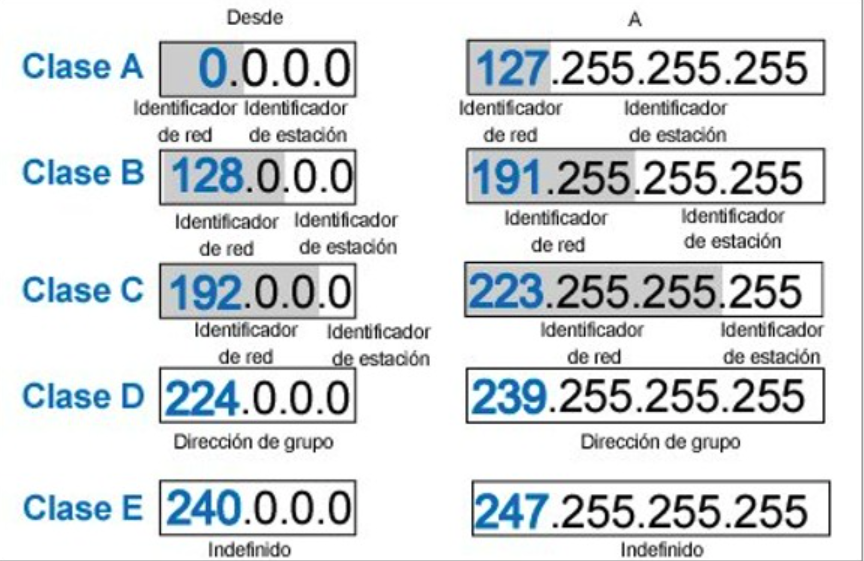
\includegraphics[width=0.6\textwidth]{images/redes 1.png}
\end{figure}


\begin{figure}[H]
    \centering
    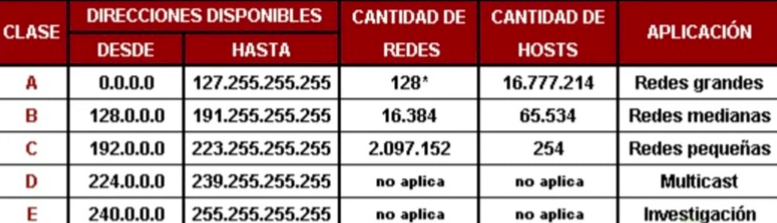
\includegraphics[width=0.7\textwidth]{images/redes2.png}
\end{figure}

La máscarada de red \textbf{NO} especifica las clases de IP, sino los \textbf{NODOS} que pueden existir en una red o subred.

\section{SUBNETEO}
Dividir una red primaria en una serie de subredes, de tal forma que cada una de ellas va a funcionar luego, a nivel de envío y recepción de paquetes, como una red individual aunque todas pertenezcan a la misma red principal y por lo tanto, al mismo dominio.
\vspace{0.3cm}\\ 
De una red generar otras subredes.

\section{Localhost}
Tiene utilidades muy interesantes, especialmente si vas a crear una página web, quieres aprender a programar o estás al cargo de una red local.

Localhost es el nombre que se usa para designar para la computadora o el dispositivo que estás utilizando en un momento determinado. Es lo que la traducción literal define como "huésped local", pero es más correcto definirlo como dispositivo local o servidor local.
\vspace{0.3cm}\\ 
Todo localhost tiene asignada la dirección IP 127.0.0.1 (o ::1 en IPv6), también llamada dirección IP de loopback o bucle reverso. Se llama así porque permite utilizar ciertas herramientas TCP/IP (relacionadas con páginas web) apuntando así misma, es decir, en modo local, sin necesidad de conectarse a internet y sin salir del ordenador.
\section{HOST}
Un host es cualquier computadora o máquina conectada a una red a través de un dominio y un número de IP definidos. Su función es proporcionarle recursos, información y servicios a los usuarios.
\newpage
\section{MÁSCARAS DE RED}
La máscara de red es una combinación de bits que sirve para delimitar el ámbito de una red de computadoras. Su función es indicar a los dispositivos qué parte de la dirección IP es el número de la red, incluyendo a la subred y qué parte es la correspondiente al host.
\vspace{0.3cm}\\ 
La máscara de red se divide en 2 partes:

\subsection{Porción de Red}
\subsection{Porción de Host}

\begin{figure}[H]
    \centering 
    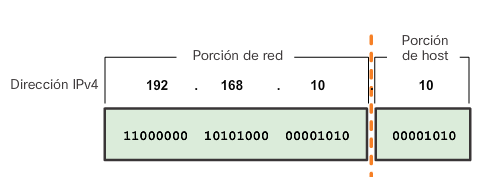
\includegraphics[width=0.7\textwidth]{redesss2.png}
\end{figure}
\begin{figure}[H]
    \centering 
    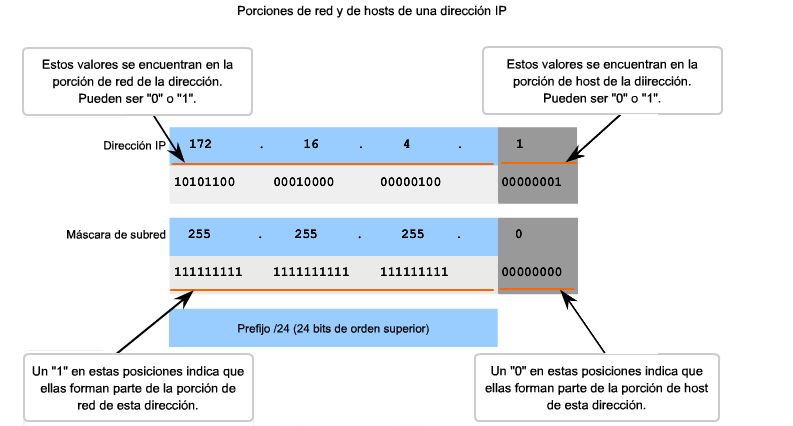
\includegraphics[width=0.7\textwidth]{redes3.png}
\end{figure}

\subsubsection{Mascaras de subred por defecto por clases}
\begin{itemize}
    \item CLASE A: 255.0.0.0
    \item CLASE B: 255.255.0.0
    \item CLASE C: 255.255.255.0
\end{itemize}

\subsubsection{SUBNETEO O SUBNETTING}
Es el proceso de dividir una red en redes más pequeñas y manejables. Las subredes se crean para evitar que el tráfico broadcast se envíe a todos los destinos de una red determinada. El exceso de broadcast consume recursos como ancho de banda, ciclos del CPU de los dispositivos, así como memoria.
\vspace{0.3cm}\\ 
Otro concepto importante en subneteo es la máscara de subred. La máscara de subred es una cantidad de 32 bits, que se expresa en formato decimal punteado; esta indica qué parte de una dirección IP pertenece a la red y la cantidad que pertenece al host.

\begin{figure}[H]
    \centering
    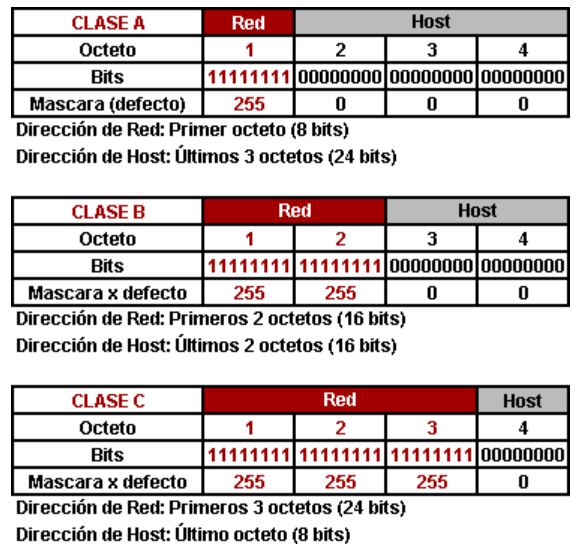
\includegraphics[width=0.7\textwidth]{redes4.png}
\end{figure}



\end{sloppypar}
\end{document}